\begin{problem}{Японский кроссворд.}{стандартный ввод}{стандартный вывод}{1 секунда}{256 мегабайт}

В данной задаче вам необходимо решить японский кроссворд. Японский кроссворд - головоломка, в которой, в отличие от обычных кроссвордов, закодированы не слова, а изображения. Изображения закодированы числами, расположенными слева от строк, а также сверху над столбцами. Количество чисел показывает, сколько групп чёрных клеток находятся в соответствующих строке или столбце, а сами числа --- сколько слитных клеток содержит каждая из этих групп (например, набор из трёх чисел --- 4, 1, и 3 означает, что в этом ряду есть три группы: первая --- из четырёх, вторая --- из одной, третья --- из трёх чёрных клеток). В чёрно-белом кроссворде группы должны быть разделены, как минимум, одной пустой клеткой. В отличии от настоящих японских кроссвордов здесь может быть несколько решений.

\InputFile
Первая строка содержит $t$ - количество кроссвордов, в следующих $t$ строках описываются кроссворды :  
На первой строке вводятся два числа $n$, $m$ - размер кроссворда. 
В следующих $n$ строках вводятся описания строк в формате : $x$(число групп в строке) и $x$ чисел описывающих строку.
В следующих $m$ строках вводятся описания строк в формате : $x$(число групп в строке) и $x$ чисел описывающих строку.

\OutputFile
Для каждого из $t$ тестов выведите ответ в виде таблички $n$ на $m$, где 1 - черный цвет, а 0 - белый.

\Example

\begin{example}
\exmpfile{example.01}{example.01.a}%
\end{example}

\Note
ответ на первый тест из условия - 
\begin{center}
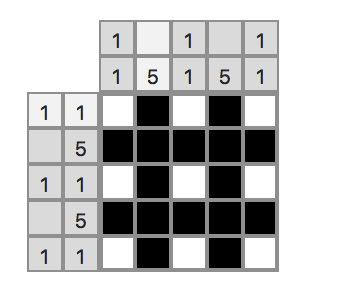
\includegraphics[width=15cm]{crossword.png}
\end{center}
За первый тест ставится от 0 до 30 баллов, за каждый кроссворд по 6 баллов.
За второй тест ставится от 0 до 70 баллов, за каждый кроссворд по 10 баллов.
Формула оценки за кроссворд - (количество угаданных горизонталей + количество угаданных вертикалей) /  (количество горизонталей + количество вертикалей)


\end{problem}

